\chapter{STATE OF THE ART}
\normalsize{In this chapter, the design, the use and the architecture of the reflector tile will be explained. Moreover, the already existing analyses and results will be discussed to give context and insight about the situation and the functionning of this system.}
\section{THE \acrshort{ECRH} \acrshort{TZM} REFLECTOR TILE ASSEMBLY}
\normalsize{The reflector tile is used to reflect the \acrshort{ECRH} beam back into the plasma to limit energy loss. This reflector tile is placed in a particular position inside of the stellarator.}
\\
\begin{figure}[h!]
    \centering
    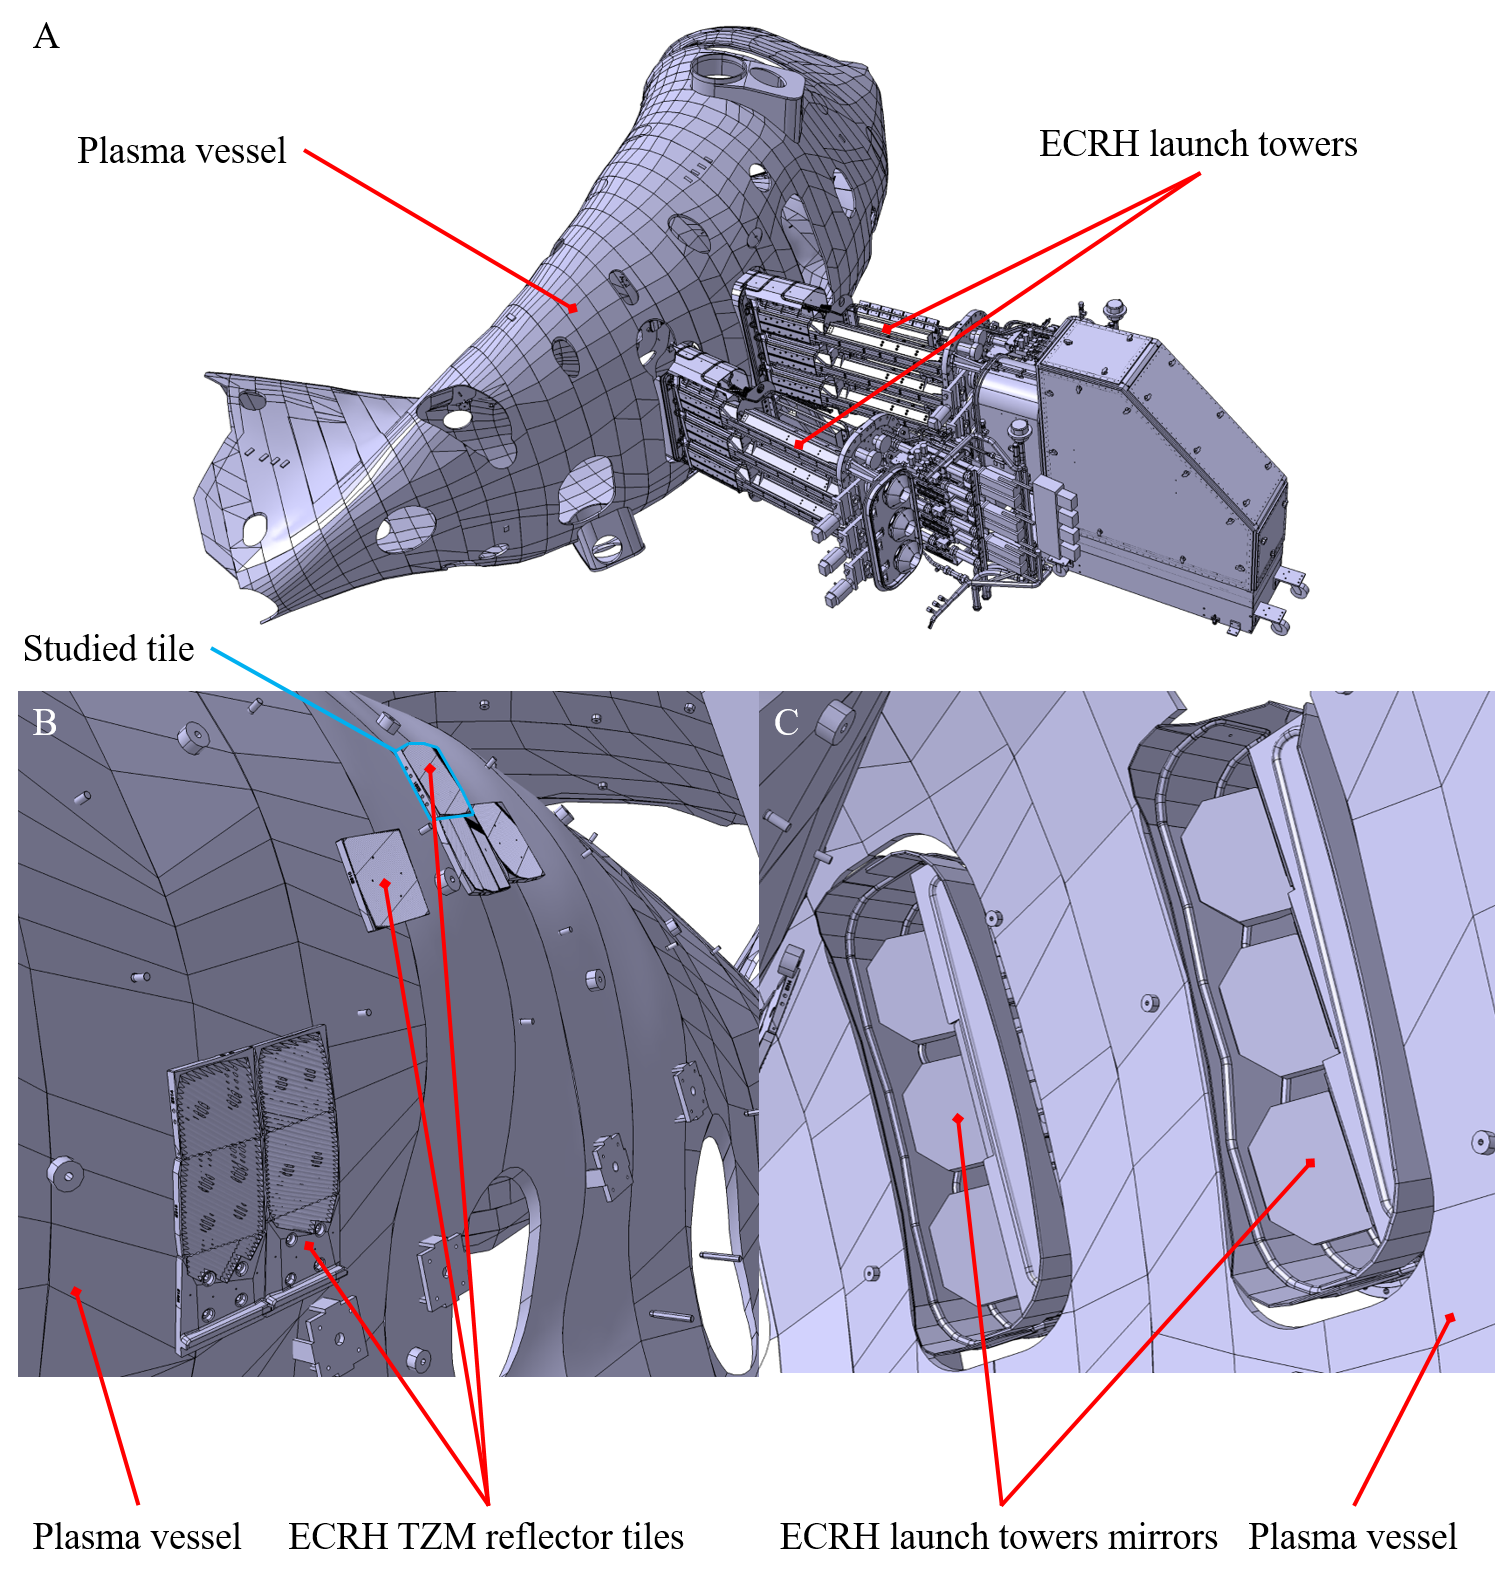
\includegraphics[width=1\textwidth]{figures/ecrhposition2.png}
    \caption{\it A: }
    %\label{fig:fig_3_1}
\end{figure}
\\
\break
\normalsize{\indent  The reflector tiles face the plasma and are a component of the \acrshort{PFCs} and are placed in front of the \acrshort{ECRH} launch towers. A reflective alloy made of titanium zirconium and molybdenum abbreviated \acrshort{TZM} was chosen to build the reflector tile. The reflector tile is mounted on a copper chromium zirconium heat sink that is brazed onto a stainless steel cooling pipe. The \acrshort{ECRH} reflector tile is placed on one of the modules composing the in-vessel components or \acrshort{KiP}.}
\\
\break
\normalsize{\indent INSER TEXT ABOUT MONTAGE}
\section{PREVIOUS ANALYSES OF THE ECRH REFLECTOR TILE}
\normalsize{In order to reflect the \acrshort{ECRH} beam into plasma back, some \acrshort{TZM} tiles were suggested to substitute the \acrshort{BM} graphite tiles in specific positions. The idea was to limit power loss due to absorption of the \acrshort{ECRH} beam by the graphite tiles. After \acrshort{OP1}.2 it was decided to increase the size of the \acrshort{TZM} tile. Due to the fact the tile has been never analyzed in details, corresponding thermal and structural analysis is to be performed to assess the performance of the tile in \acrshort{OP2}.}
\\
\break
\normalsize{\indent For \acrshort{OP2}, plasma discharge duration will be increased thus exposing the \acrshort{PFCs} to longer heat loads. The “worst” tile had been selected during discussion between V. Bykov and T. Stange and was analyzed. Those analyses aimed to give insight about the thermal and structural integrity of the \acrshort{ECRH} reflector tile during the plasma discharges with \acrshort{OP2} specifications.}
\\
\begin{figure}[h!]
    \centering
    \includegraphics[width=.45\textwidth]{figures/JFellingerFEModel.png}
    \caption{\it FE model of the tile assembly \cite{Fellinger_2013}}
    \label{fig:fig_3_2}
\end{figure}
\\
\break
\normalsize{\indent Different analyses such as transient thermal and fatigue analyses were performed by various engineers to assure proper functioning of the tile. One of those analyses were performed by J. Fellinger in 2013 and was the thermal-mechanical assessment of heat shields and baffles \cites{Fellinger_2013}. The analyses were performed on a simplified model $see figure \ \ref{fig:fig_3_1}$ of the tile and calculated using Dassault Systèmes Abaqus. Perfect thermal contact between the parts was also assumed to simplify the model. The heat pulse was simplified to be a step signal lasting for about $90 \ s$. Models for fatigue dimensionning and material properties were defined and used in this work. Thermal properties of the differents materials used are also given and important for the rest of the work.}
\\
\break
\normalsize{
\indent The conclusions of this work were that the fatigue of the steel cooling pipe.

 The plastic strain in the steel pipe under test conditions remains within the acceptable limit of $0.9 \% $ for low cycle fatigue (LCF) after 500 cycles, indicating that no failure or leakage occurred during the test. However, the plastic strain significantly exceeds the $0.2 \%$ limit for 60,000 cycles as planned for \acrshort{W7-X}.

The effect of the boundary conditions, in particular restraining the axial displacement of the the steel cooling pipe has a non-negligible and detrimental influence on the plastic strain \cites{Fellinger_2013}. This conclusion is going to be seen later in this work regarding the structural analysis.
}
\\
\break
\normalsize{\indent In this work, a discussion about the thermal performances of the brazing between the heat sink and the cooling pipe or the Sigraflex thermal gasket also stated that these moderatly affected the heat transfer within the tile assembly. On the other hand, the annealing of alloys and the temperature-dependant mechanical properties are a concern and the issue of having uncertain annealing of the \acrshort{CuCrZr} due to termal activation arose \cites{Fellinger_2013}. This will be an issue discussed later in the topic of this work.}
\\
\break
\normalsize{\indent Later, Jiawu Zhu was tasked to analyse the behavior of the tile }

\section{ISSUES OF THE TILE}
